Длинная линия — модель линии передачи, продольный размер (длина) которой превышает длину волны, распространяющейся в ней. Такая линия передачи может быть охаракетризована погонными параметрами:
$R_0$ -- погонное сопротивление, $G_0$ -- паразитная, погонная проводимость, $L_0$ -- погонная индуктивность, $C_0$ -- погонная емкость.


Рассмотрим два рядом идущих длинных провода (коаксиальный кабель, например). Тогда в $z$ и $z+ \Delta z$ ток будет различным, как и, соответсвенно, разность потенцаилов. 
\begin{equation*}
    V(z+\Delta z) - V(z) = \frac{L_0 \Delta z}{c^2} \frac{\partial I}{\partial t},
    \hspace{1cm} 
    I(z) = I(z+\Delta z) + \frac{\partial q}{\partial t},
    \hspace{1cm} 
    q = C_0 \Delta z V.
\end{equation*}

\begin{figure}[h]
    \centering
    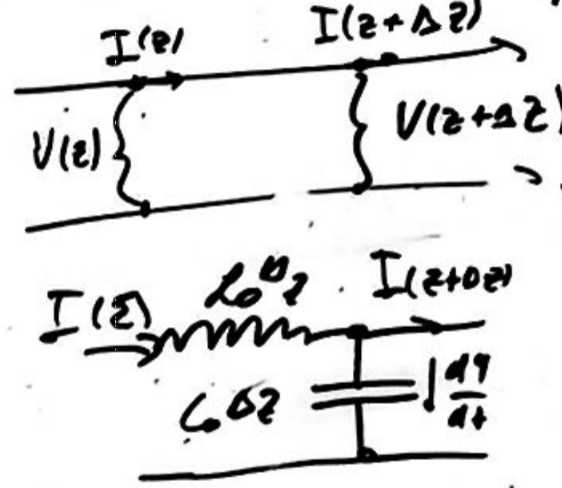
\includegraphics[width=0.25\textwidth]{img/2.png}
    %\caption{}
    %\label{fig:}
\end{figure}

\noindent
Из этих уравнений легко получить, что
\begin{equation}
    \left\{\begin{aligned}
        \frac{\partial U}{\partial z} &= - \frac{L_0}{c^2} \frac{d I}{d t} \\
        \frac{\partial I}{\partial z} &= - C_0 \frac{\partial U}{\partial t} 
    \end{aligned}\right.
    \hspace{0.5cm} \Rightarrow \hspace{0.5cm} 
    \boxed{
        \frac{\partial^2 U}{\partial t^2}  = \frac{c^2}{L_0 C_0} - \frac{\partial^2 V}{\partial z^2} 
    }.
\end{equation}
Решение аналогично будем искать в виде
\begin{equation}
    V = f_1 (z - vt) + f_2 (z + vt),
    \hspace{0.5cm} \Rightarrow \hspace{0.5cm} 
    v = \frac{c}{\sqrt{L_0 C_0}}.
\end{equation}
Кстати, если это всё посчитать для коаксиального кабеля, то
\begin{equation*}
    L_0 = 2 \mu \ln \frac{R_2}{R_1} , \hspace{0.5cm} 
    C_0 = \frac{\varepsilon}{2 \ln \frac{R_2}{R_1} },
    \hspace{0.5cm} \Rightarrow \hspace{0.5cm} 
    v = \frac{c}{\sqrt{\mu \varepsilon}}.
\end{equation*}


\subsubsection*{Коэффициент стоячей волны (standing wave ratio)}
Коэффициент стоячей волны -- отношение наибольшего значения амплитуды напряжённости электрического или магнитного поля стоячей волны в пучностях линии передачи к амплитуде в узлах.
КСВ является мерой согласования нагрузки (например, антенны) с линией передачи.

Наибольшее и наименьшее значения амплитуды соответсвенно равны
\begin{equation*}
    A_{\text{max}} = A_{\text{inc}} + A_{\text{ref}}, \hspace{0.5cm} 
    A_{\text{min}} = A_{\text{inc}} - A_{\text{ref}},
    \hspace{0.5cm} \Rightarrow \hspace{0.5cm} 
    \text{КСВ} = \frac{A_{\text{inc}} + A_{\text{ref}}}{A_{\text{inc}} - A_{\text{ref}}} = 
    \frac{1 + |\Gamma|}{1 - |\Gamma|},
\end{equation*}
где $|\Gamma|$ -- коэффициент отражения.

\subsubsection*{Согласованная нагрузка}
Рассмотрим длинную линию, пусть в цепи 
\begin{equation*}
    U = U_0 \cos \left(\omega_0 t - kz\right),  \hspace{0.5cm} 
    I = I_0 \cos \left(\omega_0 t - kz\right).
\end{equation*}
Сделаем следующий трюк. Возьмем, и продолжим линию до бесконечности, от которой, очевидно, ничего не отразится. Соотвественно нас интересует поиск эквивалентного импеданса системы. 
\begin{align*}
    U^* = U_0 \exp\left(i(\omega_0 t - kz)\right) &= U_0 e^{ikz} e^{-i\omega_0 t}, \\
    I^* = I_0 \exp\left(i(\omega_0 t - kz)\right) &= I_0 e^{ikz} e^{-i\omega_0 t}.
\end{align*}
Подставив эти выражения в волновое уравнение, и получим
\begin{equation*}
    ik U^* = i \omega_0 I^*,
    \hspace{0.5cm} 
    Z^* = U^* / I^* = \frac{\omega_0}{k},
    \hspace{0.5cm} \Rightarrow \hspace{0.5cm} 
    R = \frac{1}{c} \sqrt{\frac{L_0}{C_0}},
    \text{\ \ --- \ \ \textit{согласованная нагрузка}}.
\end{equation*}
То есть при наличии такого сопротивления на конце линии не будет никакого отражения. 


